\section{Introduction}

This lab examines the phenomenon of polarized light. You will learn what 
polarization of light is and what the polarization axis of a polarizer 
is. We will see how the intensity of the light transmitted through a polarizer 
depends on the angle between the polarization axis of the polarizer and the 
polarization vector of the incident light. We will also examine various 
combinations of polarizers.

\section{Theory}

\subsection{References}

A very brief discussion of polarization is given in Serway, Section~38.6 
(Polarization of Light Waves).

\subsection{Polarization}

In this week's lab we will explore some aspects of the wave nature of light.
Light is a transverse wave of oscillating electric and magnetic fields,
depicted in Figure~\ref{fig:pol:EMwave}.  
\begin{figure}
\centering 
\epsfxsize=7cm 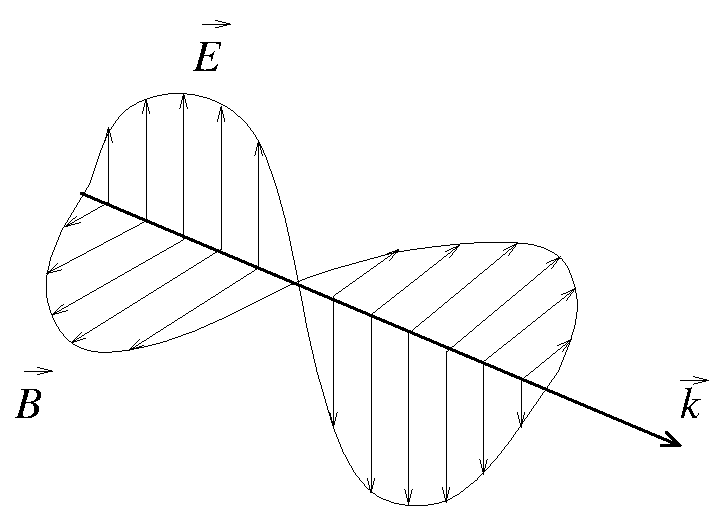
\includegraphics[scale=0.6]{7_polarization/EMwave.eps}
\caption{Light is a wave.}
\label{fig:pol:EMwave}
\end{figure}
By transverse, we mean that the electric and magnetic fields oscillate in a 
plane that is transverse, or perpendicular, to the direction that the wave is
moving or propagating. The wave vector $\vec{k}$ points in the direction of 
propagation; so transversality requires 
$\vec{k}\cdot\vec{E}=\vec{k}\cdot\vec{B}=0$. Also, as is clear from the figure,
the cross-product $\vec{E}\times\vec{B}$ points in the same direction as 
$\vec{k}$.  The intensity of the wave is given by 
$$ I = \frac{\epsilon_0}{2} |\vec{E}|^2. $$ 

What we call polarization is the measure of how the wave is oriented in 
space. So far, we know that the wave vector $\vec{k}$ tells us which way the 
wave travels;  we'd also like to know which way the oscillating fields are 
pointing. If we know the direction of both $\vec{k}$ and $\vec{E}$, the 
relation with the cross-product, namely $\vec{E}\times\vec{B}\parallel\vec{k}$,
allows us to determine the direction of $\vec{B}$.  As a convention, we define 
the {\it polarization vector} $\hat{\varepsilon}$ of the wave to be a unit 
vector in the direction of the electric field
$$ \hat{\varepsilon} =\frac{\vec{E}}{|\vec{E}|}. $$   
We could just as well have used $\vec{B}$ to define $\hat{\varepsilon}$, but 
our convention matches everyone else's and it would be nice if we could 
communicate with everyone else. Actually the reason for the convention is 
simple. For electromagnetic plane waves, the magnitudes of $\vec{B}$ and 
$\vec{E}$ are related by
$$ E=cB, $$   
where $c=2.997~924~58 \cdot 10^8$~m/s is the speed of light.  The magnitude of 
the force on a particle with charge $q$ due to the electric field of the wave 
is $F_E = qE = qcB$, while the magnetic force has a magnitude $F_M=qvB$.  
The velocity of the particle will usually be much less than $c$, so that 
$v\ll c$ and $F_E \gg F_M$. In this sense, the electric field of the light 
wave is ``stronger'' than the magnetic field, so the convention is a natural 
one.

Since $\hat{\varepsilon}$ is a vector, we can project it into components in 
some coordinate system. In Figure~\ref{fig:pol:component}, 
$\hat{\varepsilon}=\vec{\varepsilon}_x+\vec{\varepsilon}_y$. The 
$\vec{\varepsilon}_x$ and $\vec{\varepsilon}_y$ are not unit vectors. 
\begin{figure}[htb]
\centering 
\epsfxsize=4cm 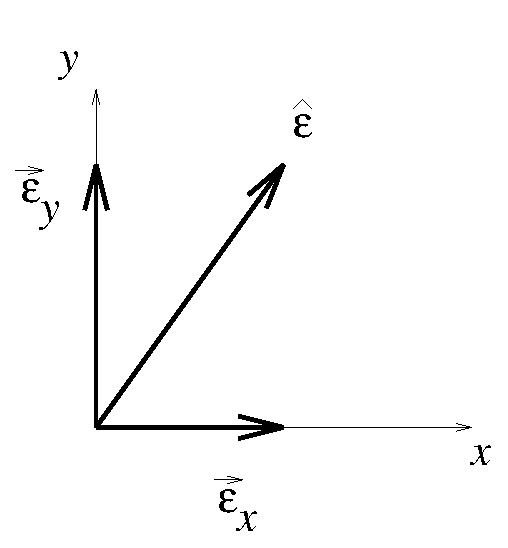
\includegraphics[scale=0.6]{7_polarization/polcomponent.eps}
\caption{A polarization vector can be split into components.}
\label{fig:pol:component}
\end{figure}
However, $\hat{\varepsilon}$ doesn't quite define a single direction. Since 
$\vec{E}$ is oscillating, it changes sign every half-wavelength.  Therefore 
$\hat{\varepsilon}$ and $-\hat{\varepsilon}$ both define the same polarization,
this is illustrated in Figure~\ref{fig:pol:polvect}. When we talk about a 
polarization vector, we really mean the two orientations denoted by 
``$\hat{\varepsilon}$'' in the figure.
\begin{figure}[htb]
\centering 
\epsfxsize=5cm 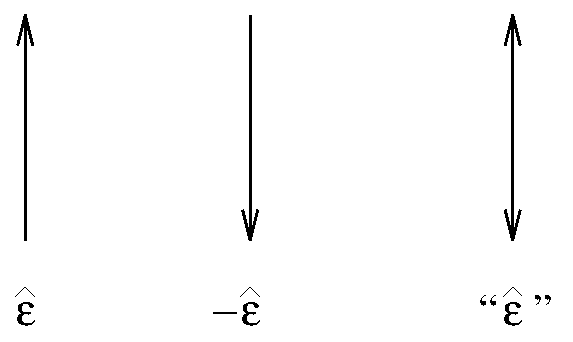
\includegraphics[scale=0.6]{7_polarization/polvect.eps}
\caption{The polarization vector refers to two directions.}
\label{fig:pol:polvect}
\end{figure}
We will be specifically interested in waves for which the polarization vector
remains along the same line as the wave propagates. These waves are called 
linearly polarized. There are more complicated situations in which the 
polarization vector rotates as the wave propagates, such as in the case of 
circular and elliptic polarization. We will not discuss these here.

We have defined what we mean by polarization for a single wave.  The light from
most sources, such as a lamp or the sun, contains more than just one wave.
The light around you is a combination of many waves.  The units of light are 
called photons.  These photons are themselves waves, so that when you put them 
together they obey the superposition principle and you get a more complicated 
wave out. Each photon will have its own polarization vector, but in general, 
the polarization vectors will not all point in the same direction.  
Superposition requires that we add the polarization vectors of all the photons 
up. They can add to give some overall polarization or they can add to give 
zero. When they add to give an overall polarization, we say that the light is 
polarized; when they give zero, the light is said to be unpolarized.  A 
typical light source, such as a lamp, will generally emit unpolarized light. 
This is because the polarization vectors of the individual photons emitted 
from a lamp are typically randomly distributed. This means that if we were to 
pick a single photon out of the sample, it would be as probable that we would 
measure its polarization vector to be in one direction in the transverse plane 
as to find it in any other.  If we were to add up all of the polarization 
vectors in the random distribution we would get zero total polarization. If we 
have polarized light, it is always most probable to find the polarization 
vector of an individual photon to be in the direction of the overall 
polarization of the light. The situation is hinted at in 
Figure~\ref{fig:pol:unpolarized}.
\begin{figure}
\centering 
\epsfxsize=7cm 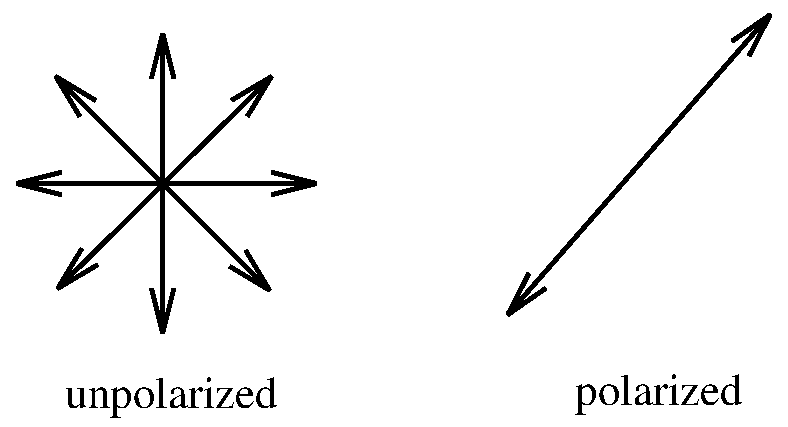
\includegraphics[scale=0.6]{7_polarization/unpolarized.eps}
\caption{Unpolarized versus polarized light.}
\label{fig:pol:unpolarized}
\end{figure}

\subsection{Polarizers}

How can we obtain polarized light from a source of unpolarized light? One
simple method that we will make use of is to use a Polaroid filter, also called
a polarizer.  Polaroid consists of plastic upon which there are long strings of
quinine iodosulfate molecules, see Figure~\ref{fig:pol:polaroid}.
\begin{figure}
\centering 
\epsfxsize=6cm 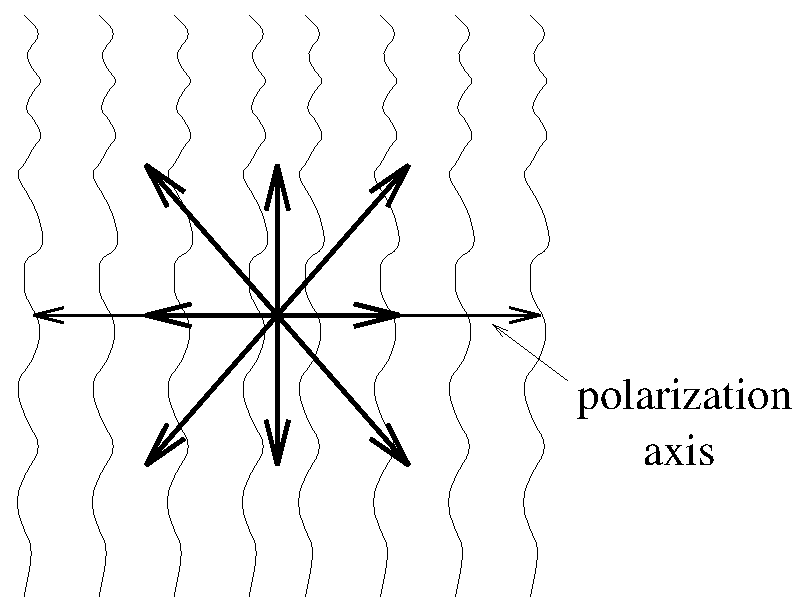
\includegraphics[scale=0.6]{7_polarization/polaroid.eps}
\caption{The polarizer transmits the component of the incident light with its 
polarization vector along the polarization axis.}
\label{fig:pol:polaroid}
\end{figure}
These molecules absorb photons with a polarization vector along the direction 
of the strings. This is because their electric fields oscillate along the 
strings and easily excite the electrons in the molecules and are therefore 
absorbed.  Some of the remaining photons, namely those with a polarization 
vector close to the direction of the string, are absorbed as well. The photons 
that are actually transmitted are those whose polarization vector is nearly 
perpendicular to the strings, so that the resulting light has a strong 
polarization in the direction perpendicular to the strings. This perpendicular 
direction is called the polarization axis of the polarizer. Another way we'll 
use to illustrate how a polarizer works is that in 
Figure~\ref{fig:pol:transmit}.
\begin{figure}
\centering 
\epsfxsize=8cm 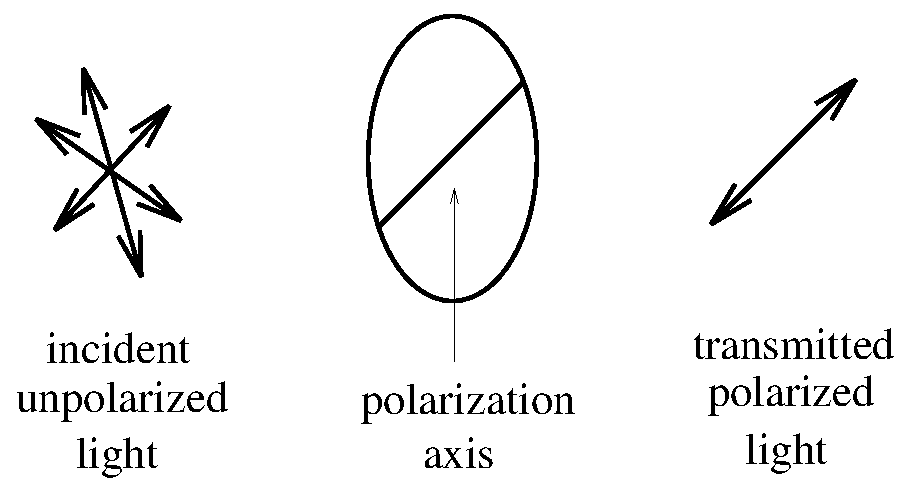
\includegraphics[scale=0.6]{7_polarization/transmit.eps}
\caption{Another illustration of a polarizer.}
\label{fig:pol:transmit}
\end{figure}

\subsection{Malus' Law}

The light that gets through the polarizer will be reduced in intensity, simply
because only the photons with a component of polarization in the direction of 
the polarization axis get through. We would now like to get a quantitative 
measure of the transmitted intensity.  We will first deal with polarized light 
incident on a polarizer. In Figure~\ref{fig:pol:malus}, the electric field 
vector $\vec{E}$ of the incident light is shown projected onto the 
polarization axis of the polarizer. The magnitude of the electric field for 
the transmitted light is just the component of $\vec{E}$ along the 
polarization axis,
$$ E_{\mbox{trans}} = E \cos\theta, $$
where $\theta$ is the angle between the polarization vector of the incident 
light and the polarization axis of the polarizer. 
\begin{figure}[hb]
\centering 
\epsfxsize=6cm 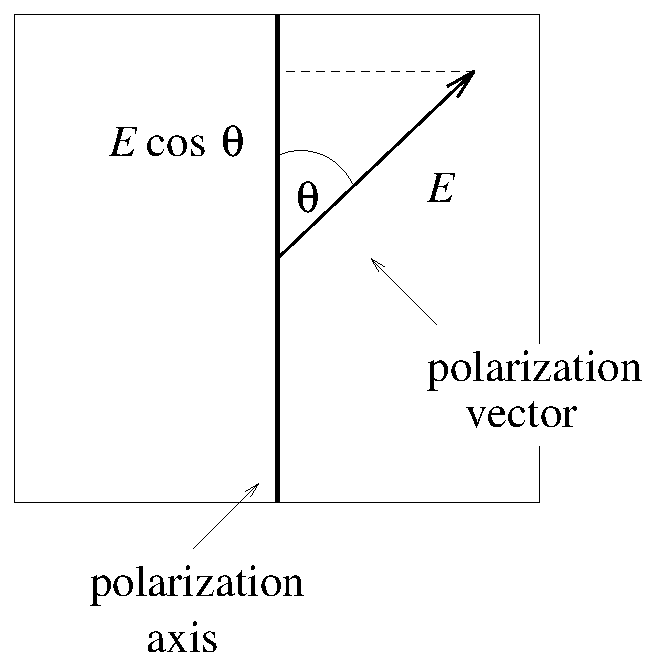
\includegraphics[scale=0.6]{7_polarization/malus.eps}
\caption{The sketch used to derive Malus' law.}
\label{fig:pol:malus}
\end{figure}
The transmitted intensity is
\begin{eqnarray*}
I &=& \frac{\epsilon_0}{2} |E_{\mbox{trans}}|^2  \\
&=& \frac{\epsilon_0}{2} |E \cos\theta |^2   \\
&=& \left( \frac{\epsilon_0}{2} |E|^2 \right) \cos^2\theta  \\ 
&=& I_0 \cos^2\theta,
\end{eqnarray*}
where we have identified the intensity of the incident light as $I_0$.

The result: \\
\begin{equation}
\fbox{$ \displaystyle I = I_0 \cos^2\theta, $} \label{eq:pol:maluslaw}
\end{equation}
is called Malus' law. It is the only 
equation we need to discuss the results for this lab. However, as is clear from
how we went about deriving it, it only applies to the case where the incident
light is polarized. We would like to know what the transmitted intensity will
be if the incident light is unpolarized. If we recall the discussion about
unpolarized light consisting of photons with randomly distributed polarization
vectors, since each photon is polarized we can average Malus' law over all of 
the contributions to the final intensity. Since there are $2\pi$ radians in a 
circle, the transmitted intensity, as given by Malus' law, is
\begin{eqnarray*}
I &=& \frac{1}{2\pi} \int_0^{2\pi} I_0 \cos^2\theta d\theta \nonumber \\
I &=& \frac{I_0}{2}.
\end{eqnarray*}
Half of the incident unpolarized light will get through the polarizer. 

\section{Apparatus}

We will be using lamps as white light sources. The light should be, for the 
most part, unpolarized, but you will make measurements to determine if this is 
in fact the case.  The polarizers are marked with angles. The polarization
axis of the polarizers runs from the $0^\circ$ marking to the $180^\circ$ 
marking.  We'll place the polarizers in magnetic mounts during use. There
is a white mark at the base of the mounts which clearly indicates the angle 
between the polarization axis of the polarizer and vertical.

To measure the intensity of light that is transmitted through the polarizers, 
we will use a photodetector.  The photodetector absorbs the light that falls
on it and registers a voltage that you can read on a voltmeter. This voltage
is directly proportional to the intensity of the light incident on the 
photodetector, $V\propto I$.  We will only be studying {\it changes} in the
transmitted intensity versus changes in the angle settings of the polarizers,
and so we do not need to measure the constant of proportionality. A change in 
the voltage signals a proportional change in the intensity.  An important
property to note is that the photodetector must be connected to its power 
supply (in our case, a battery) in the proper direction, connect the {\it red} 
lead to the {\it positive} pole of the battery and the {\it black} to the 
{\it negative} pole.

\vfill
\pagebreak
$$
$$
\vfill
\clearpage
\newpage

%  Label worksheets by \thechapter.W
\renewcommand{\thesection}{\thechapter.W}

\section{Polarization of Light Worksheet}
{\bf \Large Name:}~ \rule{5cm}{.1mm}~~~~~~~
{\bf \Large Day/Time:}~\rule{3cm}{.1mm}\\
{\bf \Large Partner's Name:}~\rule{6cm}{.1mm}\\
\subsection{In-Lab Procedure}
\label{sec:pol:proc}

It is important that you do not move the lamp during the course of 
data taking. Take care to leave the lamp in the same position for all 
measurements during a given procedure.  You will probably also find it helpful
to tape down the magnetic stands so that they don't move during 
measurements either.

\subsubsection{Preliminaries}

You should begin by connecting the photodectector to the multimeter. 
Set the multimeter to record voltage. Set the polarizers on the magnetic 
stands.  There is a white mark at the base of the stand to allow you to 
measure the angle of the polarizer. \\

\noindent Set one polarizer directly in front of the photodetector. In this
and all following parts of the procedure make sure that the gaps between
the polarizers and the photodetector are as small as possible and that 
the lamp is as close as possible to the first polarizer. The set-up is 
illustrated in Figure~\ref{fig:pol:onepol}
\begin{figure}[htb]
\centering 
\epsfxsize=7cm 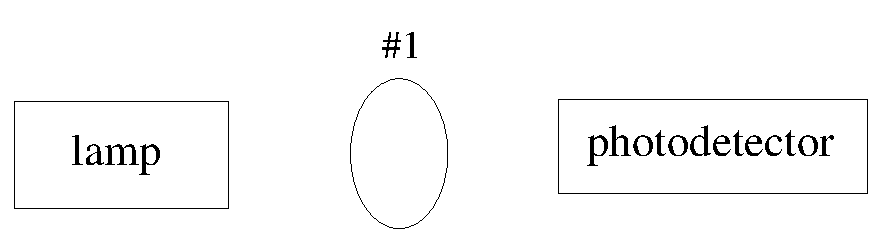
\includegraphics[scale=0.6]{7_polarization/onepol.eps}
\caption{Is the light from the lamp polarized?}
\label{fig:pol:onepol}
\end{figure}

\noindent Record the voltage displayed.  
Watch the display for a few seconds. Does 
the voltage value change? If so, record the maximum and minimum values taken. 
Add half of the difference in these values to the uncertainty in 
your voltage values and claim the sum obtained as the uncertainty in all
of the following voltage measurements. This accounts for any fluctuations in
the voltage produced by the photodiode. Remember that the voltage, $V$, is 
directly proportional to the intensity, $I$, of the light falling on the 
polarizer. \\

\noindent For the above set-up measure the voltage, $V$, 
for five well separated 
polarizer angles, $\theta$, in the range $0^\circ$ to $90^\circ$.  Enter the 
voltage and angle values with uncertainties into Table~\ref{tab:PO:1lens}.

\begin{table}[htb]
\begin{center}
\begin{tabular}{|c|c|}
\hline
\multicolumn{2}{|c|}{Measurements of $V$ vs. $\theta$} \\
\hline
Voltage, $V$ & Angle, $\theta$  \\
\hline
\hspace*{3cm} & \hspace*{3cm}  \\
&   \\
\hline
&   \\
&  \\
\hline
& \\
& \\
\hline
&  \\
&  \\
\hline
&  \\
&  \\
\hline
\end{tabular}
\end{center}
\caption{$V$ vs. $\theta$ measurements for single polarizer}
\label {tab:PO:1lens}
\end{table}


\subsection{In-Lab Computer Work}

Plot $V$ vs. $\theta$ on KaleidaGraph.  Is the plot linear within error?  
If it is, then 
fit the line with curve fit1. 

\subsection{In-Lab Procedure}
\subsubsection{Polarized Light and a Polarizer}

Place a second polarizer between the first polarizer and the 
photodetector, as in Figure~\ref{fig:pol:twopol}. 
\begin{figure}[htb]
\centering 
\epsfxsize=8cm 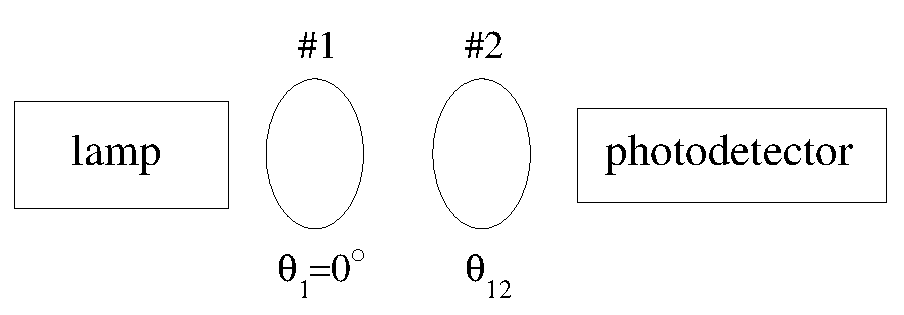
\includegraphics[scale=0.6]{7_polarization/twopol.eps}
\caption{Set-up for testing Malus' law.}
\label{fig:pol:twopol}
\end{figure}

\noindent Set the polarization angle of the first 
polarizer (\#1), $\theta_1$, to zero.  
Measure the angle that the polarization axis of the 
second polarizer (\#2) makes with that of the first, $\theta_{12}$, 
{\it relative} to $\theta_1$.  
Measure $V$ vs. $\theta_{12}$ for $10^\circ$ increments from $0^\circ$ to 
$90^\circ$.  
Enter these values with uncertainties into Table~\ref{tab:PO:2lens}.

\begin{table}[htb]
\begin{center}
\begin{tabular}{|c|c|c|c|c|}
\hline
\multicolumn{5}{|c|}{Measurements of $V$ vs. $\theta _{12}$ for
 Two Polarizers.} \\
\hline
Voltage, $V$ & Angle, $\theta _{12}$ & & Voltage, $V$ & Angle, $\theta _{12}$\\
\hline
\hspace*{3cm} & \hspace*{3cm} & \hspace*{.3cm} & \hspace*{3cm} & \hspace*{3cm}
\\
& & & & \\
\hline
& & & & \\
& & & & \\
\hline
& & & & \\
& & & & \\
\hline
& & & & \\
& & & & \\
\hline
& & & & \\
& & & & \\
\hline
\end{tabular}
\end{center}
\caption{$V$ vs. $\theta _{12}$ measurements for two polarizers.}
\label {tab:PO:2lens}
\end{table}



\subsection{In-Lab Computer Work}
Plot $V$ vs. cos$^2\theta_{12}$ with error bars.  Is the plot linear?  If it is, then 
fit the line.  Show your work in obtaining the uncertainty in cos$^2\theta_{12}$ in the space provided here. \\
\vspace*{2.5cm}

\subsection{In-Lab Procedure}
\subsubsection{Crossed Polarizers}
\label{sec:pol:crosspol}

Now place a third polarizer (\#3) between the second polarizer and 
the photodetector, as in Figure~\ref{fig:pol:threepol}.  
\begin{figure}[htb]
\centering 
\epsfxsize=9cm 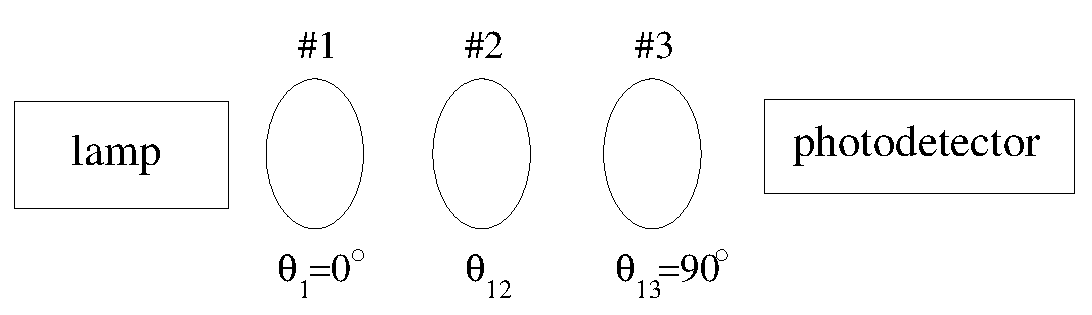
\includegraphics[scale=0.6]{7_polarization/threepol.eps}
\caption{Three polarizers.}
\label{fig:pol:threepol}
\end{figure}
Set the angle of the polarization axis of this polarizer to be perpendicular 
({\it i.e.}, at a $90^\circ$ angle to) that of the first polarizer.  \\

\noindent 
Again, 
measure $V$ vs.
$\theta_{12}$ for $10^\circ$ increments from $0^\circ$ to $90^\circ$.  
Remember that you need to vary the {\it middle} polarizer, \#2.
Enter the values for $V$ and $\theta_{12}$ into Table~\ref{tab:PO:3lens}.
 
\begin{table}[htb]
\begin{center}
\begin{tabular}{|c|c|c|c|c|}
\hline
\multicolumn{5}{|c|}{Measurements of $V$ vs. $\theta _{12}$ for
 Three Polarizers.} \\
\hline
Voltage, $V$ & Angle, $\theta _{12}$ & & Voltage, $V$ & Angle, $\theta _{12}$\\
\hline
\hspace*{3cm} & \hspace*{3cm} & \hspace*{.3cm} & \hspace*{3cm} & \hspace*{3cm}
\\
& & & & \\
\hline
& & & & \\
& & & & \\
\hline
& & & & \\
& & & & \\
\hline
& & & & \\
& & & & \\
\hline
& & & & \\
& & & & \\
\hline
\end{tabular}
\end{center}
\caption{$V$ vs. $\theta _{12}$ measurements for three polarizers.}
\label {tab:PO:3lens}
\end{table}

\subsection{In-Lab Computer Work}

Plot $V$ vs. $\theta_{12}$ with error bars.  Is the plot linear?  If it is, then 
fit the line. 

\subsection{Pre-Classroom Check List}
$\bigcirc$ \hspace*{1cm} Table~\ref{tab:PO:1lens} completed with units and uncertainties \\
$\bigcirc$ \hspace*{1cm} Table~\ref{tab:PO:2lens} completed with units and uncertainties \\
$\bigcirc$ \hspace*{1cm} Table~\ref{tab:PO:3lens} completed with units and uncertainties \\
$\bigcirc$ \hspace*{1cm} 3  Plots labeled completely and correctly \\
$\bigcirc$ \hspace*{1cm} Each student has her/his own plots and worksheet \\

\subsection{In-Classroom Discussion}

Is the light from the desk lamp polarized before it encounters a polarizer? Discuss
how you can determine this from the plot you made from the data you took in the first
part of the procedure.
\vspace*{4cm}

\noindent
Is the data you took in the second part of the procedure consistent with Malus' Law (the theoretical relationship between 
the transmitted intensity and the initial intensity for polarized light passing
through a polarizer at some relative angle)?
Explain.
\vspace*{4cm}

\noindent
How can the intensity of the light passing through three polarizers be non-zero when
the first and third polarizers are perpendicular? Assume ideal experimental conditions.
\vspace*{14cm}

\noindent
For the polarizer set-up of $\S$~\ref{sec:pol:crosspol} above, show that the 
correct expression for the intensity detected by the photodetector as a 
function of $I_0$ (intensity out of the lamp) and $\theta_{12}$ is 
\begin{equation}
I=\frac{I_0}{8}\sin^2(2\theta_{12})  \label{eq:pol:addq}
\end{equation}
Do this by expressing $I_1$ (intensity after the first polarizer) in terms of 
$I_0$, $I_2$ (intensity after the second polarizer) in terms of $I_1$
and $\theta_{12}$, and $I$ (final intensity) in terms of $I_2$ and the 
relative angle between polarizers 2 and 3, $\theta_{23}$.  You will need to 
use the fact that $\theta_1$ and $\theta_{13}$ differ by $90^\circ$. 
Figure~\ref{fig:pol:threepolintens} might help.
\begin{figure}[htb]
\centering 
\epsfxsize=11cm 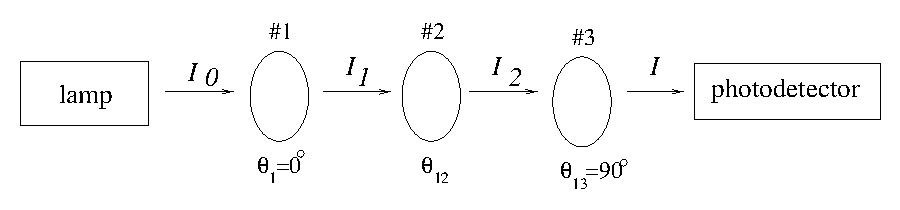
\includegraphics[scale=0.8]{7_polarization/threepolintens.eps}
\caption{Three polarizers with the intensities referred to marked.}
\label{fig:pol:threepolintens}
\end{figure}
	

\noindent {\bf Show all your work} \\
\clearpage
\noindent
Sketch $I/I_0$, given by equation~(\ref{eq:pol:addq}), versus $\theta_{12}$ 
from $0$ to $\pi/2$ and compare this profile with the graph of $V$ versus 
$\theta_{12}$ in $\S$~\ref{sec:pol:crosspol} above. 






\newpage
\subsection{In-Classroom Conclusion}

Write a {\it brief} (that is, a one or two paragraph) conclusion for
this lab. In it, you should summarize the physical
principles which were meant to be illustrated in this experiment. You
should also describe the degree to which your data supported these
principles.



\vfill
\noindent Attach plots to the worksheet. \\
\ \\
{\Large End Worksheet} 




% Go back to ordinary section numbering
\renewcommand{\thesection}{\thechapter.\arabic{section}}





